\chapter{Simulations with the \pkg{specsim} package}

Introduction: used to generate simulations for eBOSS Lyman-alpha and to verify DESI sky model. 

\section{\pkg{specsim}}

\pkg{specsim} (cite) is a software package developed by Dr. David Kirkby to simulate the response of a multi-fiber spectrograph. Although it was originally created to generate realistic synthetic spectra for the DESI instrument, it can be reconfigured to simulate any fiber-fed spectrograph, provided that the accompanying instrument parameter specifications and data are provided. 

A single simulation consists of three components: a source spectrum, a model of the sky and atmosphere, and a model of the instrument. A schema of where each component comes into play is shown in Fig. \ref{fig:overview}, which shows the journey of photons as they are emitted from a galaxy to the moment they are read out by the detector. 

%Source
Spectra of astrophysical sources are simulated individually beginning with an input spectrum in its rest frame, given in units of flux density as a function of wavelength. The source type (quasar, emission line galaxy, etc.) or profile determines whether the fiberloss method, which calculates the fraction of light incident on each fiber that makes it through, uses a pre-computed table of fiberloss fractions based on the source type, or whether it uses information about the transverse profile of the source on the sky to calculate fiberloss fractions via the \pkg{galsim} package (cite). Configuration parameters for a source profile include the bulge/disk fraction and shape parameters for each, such as the half-light radius, position angle, and the ratio of the semi-minor to semi-major axis. 

%Sky
The next piece of the \pkg{specsim} pipeline is the sky model, which incorporates the effects of the atmosphere, consisting of a sky emission spectrum, the atmospheric point spread function, or PSF, and atmospheric extinction. The sky model used for both DESI and eBOSS configurations is identical. The DESI configuration contains data for three different types of sky emission spectra corresponding to dark, bright and grey conditions, while the sky spectrum used for eBOSS is effectively the DESI dark sky extrapolated to cover the wider wavelength range of the eBOSS spectrograph.


% Give some background on seeing, what causes it, how it affects the path of a photon
Atmospheric seeing, or PSF, is the blurring of a source due to constantly changing indices of refraction in different layers of the Earth's atmosphere. This is caused by differences in temperature, pressure, density and molecular composition in each layer, as well as turbulence in the air, all of which cause photons to slightly deflect from their original paths and 'smear' a source. Seeing is measured as the FWHM from the peak value of a radial profile of a point source, which is typically a star.

The effects of atmospheric seeing in \pkg{specsim} are applied in one of two ways. If \pkg{specsim} is configured to use \pkg{galsim} as its fiberloss method, then it will also use \pkg{galsim} to calculate the seeing by requiring certain configuration parameters to be set. Because seeing $\sigma$ is assumed to scale with wavelength in the following way, 

\begin{equation}
    \sigma(\lambda) = \sigma_{ref} \Big(\frac{\lambda}{\lambda_{ref}}\Big)^{-0.2},
\end{equation}

where $\sigma_{ref}$ and $\lambda_{ref}$ are the reference FWHM and wavelength, respectively, these two parameters must be specified in the configuration file. A third required parameter is the $\beta$ parameter for the Moffat profile, the distribution used for modeling PSFs (as they are more successful at capturing tails in the PSF compared to a Gaussian or Lorentzian distribution).   

The final component in the sky model is atmospheric extinction, which could be caused by Rayleigh scattering of air molecules or particulate matter such as aerosols, or telluric absorption due to the Earth's atmosphere. This is provided in the configuration file as a list of tabulated values for the extinction coefficient at zenith as a function of wavelength. The spectral flux density $f(\lambda)$ 

attenuation of incident light, $I_{0}$, is then calculated using the extinction coefficient and airmass in the following way:



Given a source, \pkg{specsim} first incorporates the effects of sky brightness, atmospheric extinction, and the atmospheric 


in the form of extinction data and also conditions based on the location of the telescope

talk about wavelength grid under instrument (used for interpolation) - the grid used for simulation needs to be within the range of the input source grid (and all instrument data files for throughput, resolution, etc).  

\begin{figure}
\centering
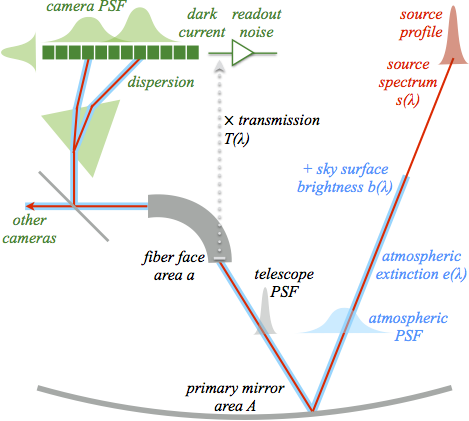
\includegraphics[width=11cm]{images/specsim/overview.png}
\caption{Specsim schema.}
\label{fig:overview}
\end{figure}

\section{Simulating the eBOSS instrument response}

\begin{table}
\caption{Instrument parameters: DESI vs eBOSS.}
\label{tab:comparison}
\centering
\begin{tabular}{|c|c|c|}
  \hline
  Instrument Parameters & DESI & eBOSS\\
  \hline \hline
  Primary mirror diameter (m) & 3.797 & 2.5 \\
  \hline
  Obscuration diameter (m) & 1.8 & 0.625 \\
  \hline
  Fiber diameter ($\mu m$) & 107.0 & 120.0 \\
  \hline
  Field radius (mm) & 414.0 & 325.0 \\
  \hline
\end{tabular}
\end{table}\\


\section{eBOSS mocks for Lyman-alpha studies}

Lyman-alpha working group needed realistic simulations of eBOSS spectra. London mocks vs saclay mocks

\section{Verifying the (ESO) sky model}


%%% Local Variables: ***
%%% mode: latex ***
%%% TeX-master: "thesis.tex" ***
%%% End: ***
